\bartchapterimage{simudm}
\bartthumb{thumb_simudm}
\chapter{Generate mock catalogues}
%
\section{Introduction}
%
\comments{Add things to this section!}A mock catalogue is a useful tool to test
algorithms involving galaxies in order to see if it is operational in a
realistic situation. Many of the properties of galaxy surveys can be simulated:
the spatial clustering of galaxies, luminosity function, incompleteness and
measures errors are some examples of them. There are different methods to
obtain such a mock catalogue. All of them involves cosmological simulations and
there halos of dark matter. According to the model of galaxy formation, we can
use halo occupation distribution (HOD) to populate dark matter haloes with
galaxy and putting some LF as constraint. We can too follow galaxies in semi
analytical models (SAM) in those cosmological simulations outputs in order to
have statistical properties of galaxies which agree with observational results.
Then with such realistic galaxies we can use those simulation boxes to place an
observer into it and create a mock survey. But to have a realistic mock
catalogue, it's necessary to take care of many things which will be described
in the next section.
%
\section{Mock structure}
%
In all this section, we will assume that we have already in our possession a
dark matter simulation box which has been populated with galaxies with one of
the methods described below (SAM, HOD\ldots). At this step, physical properties
of those galaxies aren't interesting.
%
\subsection{Placing boxes}
%
The first step to make a mock catalogue is to get galaxies positions like in a
survey, to get an $(\alpha,\delta)$ frame to simulate the sky coverage of
survey and, at the same time, project galaxies on the sky, masking to us some
spatial modulations of galaxy properties.

We want that a false observer see the same volume extension that a true survey.
For example for the SDSS survey, we can measure redshift to a value of 0.3 (and
more!). But the problem is that the majority of the simulation boxes have a
size of around $L_{\mathrm{box}}=100-300 h^{-1}$ Mpc, letting us
with a maximal redshift in our false survey of around
${H_0}{L_{\mathrm{box}}}/c\approx 0.025$ in the case of a box of
$100 h^{-1}$ Mpc sized. Bigger simulations exist, and maybe can allow us
to access to bigger redshifts, but this increasing size reduces the resolution
of the simulation in particle mass and therefore we can't have low mass halos
in the simulations.

The solution is to take a ``little'' simulation box and to replicate it and to
make some bigger ``Tetris'' cube until we reach the maximal redshift we want.
An example of the resulting ``mock cube'' is shown on figure
(\ref{fig:cubemock}).
%
\begin{wrapfigure}{l}{0.4\linewidth}
    \centering
    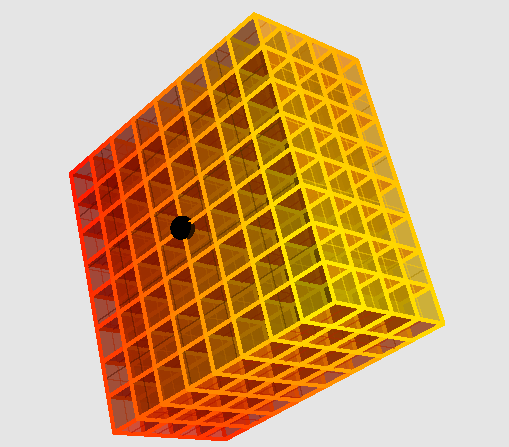
\includegraphics[width=\linewidth]{figures/mock/mock}
    \caption{The structure of the mock catalog once we have replicated the
    simulation box chosen to populate dark matter halos.}%
\label{fig:cubemock}
\end{wrapfigure}

Now if we take an observer at some position into this big box, we can have
different sky coverage for the observer. The simplest is to place the observer
at a corner which we give a solid angle of $\pi/2$ steradians. At the centre,
we have a full sky coverage but we reduce the redshift extension by 2.
%
At this time we don't care about a redshift evolution of galaxies for the
observer, but if we want to care about it, we need to use other snapshots at
different redshifts. Box sizes are similar in comobile coordinates, and
different in physical coordinates due to the variation of the Hubble constant
with redshift ($h$ depends en $z$). So juxtaposing cubes isn't as easy as the
case without redshift evolution.\comments{Maybe add details if I use it
later\ldots}
%
Many simulations give coordinates in units of $h^{-1}\mathrm{Mpc}$ but we place
galaxies in the mock in physical positions which we can measure. So coordinates
in the mock catalog are scaled to get positions in units of $\mathrm{Mpc}$.

Placing boxes as described previously can create a perspective effect from the
point of view of an observer, and the consequences aren't predictable in a
statistical sense when we try to use the mock catalog. To avoid this, we apply
some transformations on galaxies in the initial cube like inversions, rotations
and periodic translations. Rotations are multiples of $\pi/2$ around the three
principal coordinates axes, because if other rotations are allowed, it can
create some over-densities in some regions of the final mock which aren't
physical. An example of such a problem is illustrated in figure
(\ref{fig:rotation}). Translations are performed on the three principal axes
and when galaxies are out of the initial cube, periodic conditions are applied.
All of those transformations are randomly generated for each cube in the final
mock catalog.
%
\subsection{Physics}
%
We have now galaxies in a realistic coverage of the Universe, restricted to a
given volume. But an observer can't use it because galaxies are seen in
projection and he doesn't have any idea of the real distance of galaxies from
him in a statistical sense. So we need to add physic and errors to those
galaxies.
%
\subsubsection{Survey mask}
%
When studying galaxies in a survey, we are confronted to the problem of the
area of this survey. Limits are not defined in a easy analytical way in many
cases which can create some problems to correct for observers. The first step
to simulate this is to transform cartesian coordinates in the 3D space to
celestial coordinates ($(\alpha,\delta)$ frame). Get these coordinates is the
same as to compute spherical coordinates.
%
\begin{equation}
    \alpha=\left\{ \begin{array}{lcr}
     \mbox{arctan2}(Y,X)+2\pi & \mbox{if} & Y>0 \\
     \mbox{arctan2}(Y,X) & \mbox{else} & \\
    \end{array}\right.\nonumber%
\end{equation}
%
\begin{equation}
    \delta=\mbox{sign}(Z)\arccos\left(\frac{\sqrt{X^2+Y^2}}{\sqrt{X^2+Y^2+Z^2}}\right)
\end{equation}
%
In our case, the origin of coordinates is the observer. If we keep the distance
as calculated previously, the observer can still have precise determination of
the distance of a galaxy. In reality, we observe it in redshift space so the
redshift as distance indicator is biased by peculiar velocities. Our initial
galaxy catalog allow us to get the velocity of a galaxy, so we can compute the
line of sight (los) velocity of this galaxy relatively to the observer.
%
\begin{equation}
    v_{\mathrm{los}}=\cfrac{\vec{OG}.\vec{v_{\mathrm{pec}}}}{||\vec{OG}||}
\end{equation}
%
where $O$ is the observer and $G$ the galaxy, $\vec{v_{\mathrm{pec}}}$ its
peculiar velocity. This velocity has a sign. The redshift is just the
expression a shift in wavelength due to a velocity. The observed wavelength
$\lambda$ is linked to the original (emitted) wavelength $\lambda_0$ by:
%
\begin{equation}
    \lambda=(1+z)\lambda_0
\end{equation}
%
The shift caused by Universe expansion is
$\lambda_{\cos}=(1+z_{\cos})\lambda_0$ where the subscript
$\cos$ refer to the cosmological expansion. The shift caused by the
peculiar velocity is $\lambda=(1+z_{\mathrm{pec}})\lambda_{\cos}$. So
the observed wavelength is
$\lambda=(1+z_{\mathrm{pec}})(1+z_{\cos})\lambda_0$. The resulting
observed redshift is just:
%
\begin{equation}
    (1+z)=(1+z_{\mathrm{pec}})(1+z_{\cos})
\end{equation}
%
expansion. The peculiar redshift is the just due to the relativist Doppler
effect:
%
\begin{equation}
    (1+z_{\mathrm{pec}})=\sqrt{\cfrac{1+\beta}{1-\beta}}
\end{equation}
%
with $\beta={v_{\mathrm{los}}}/{c}$. The cosmological redshift is approximated
by $z_{\cos}={H_0}{D}/c$ where $D$ is the physical distance of the
galaxy to the observer and $H_0$ the Hubble constant. \comments{I think we need
    to add the velocity of the Local Group in the redshift, because in our case
the observer has a null velocity. Maybe corrected in SDSS data?}Applying this
method to the galaxies in the mock catalog, we can have galaxies whose distance
is biased by peculiar velocities in redshift space. With such a treatment, the
velocity dispersion of galaxies in groups leads to the apparition of ``fingers
of God'' as seen in observations in redshift space.

With our frame in redshift space relative to the observer, we can apply
different masks on angular coordinates according to the survey we want to
mimic. An example of such a mask is in appendix (\ref{ap:sdss}).
%
\subsubsection{K-corrections}
%
In reality, an observer study galaxies in a given bandwidth in wavelength and
can't use the bolometric flux of the object. With the expanding Universe, all
the spectral energy distribution (SED) of galaxy is shifted. All wavelengths
are shifted by the same value for a given redshift. So, knowing the luminosity
$L$ of a galaxy in a given band in reality (using the true SED), computing its
apparent magnitude for an observer isn't as easy as correcting for the distance
modulus. The observer in the same band sees a different part of the true SED\@.
The flux observed in the same band as the true flux is maybe higher or lower. A
correction for this effect is needed and must be taken into account in our mock
catalogue.

As explained before, this correction depends on the SED of galaxies and the
band used in the survey. The common way of correcting it when we have a
multi-band photometry is to fit the observed SED in those bands with
theoretical templates of SEDs. Such templates can be obtained with existing
programs as PEGASE \comments{Add references}, which give us SEDs with some
assumptions on the galaxy. But those programs are a little time consuming,
which can be a problem for mock when we want to run several of them. A good
solution is given by \citet{CMAZ10}, where the K-correction is fitted on
templates for SED as given by PEGASE in terms of a polynomial of the redshift
of the galaxy and its colour. The corresponding K-correction is precise for
redshifts until 0.3 in different survey bands (including $ugriz$ for the SDSS).
This work reduces the computation of K-corrections to the use of simple
polynomial relations and make easier our task.

By definition, the K-correction $K$ for a galaxy of apparent magnitude $m_X$ in
a given band $X$ and absolute magnitude $M_X$ in the same band is:
%
\begin{equation}
    {m_X}={M_X} + {5\log_{10}\pg{d_{\mathrm{lum}}\left[pc\right]}\pd} - 5 + K
\end{equation}
%
In our case, the K-correction depends on the redshift of the galaxy and its
colour in apparent magnitude given two bands. So we can rewrite:
%
\begin{equation}\label{eq:appmag}
    m_X = M_X + 5\log_{10}\pg{d_{\mathrm{lum}}\left[pc\right]}\pd - 5 + K( z, m_X - m_{X'} )
\end{equation}
%
where:
%
\begin{equation}
    K(z,m_{X}-{m}_{X'})=\sum_{i=0}^{N_i}\sum_{j=0}^{N_j}{a_{ij}}{z^i}{{(m_X-{m}_{X'})}^j}
\end{equation}
%
and $a_{ij}$ is a ${N_i}\times{N_j}$ matrix containing the coefficients of the
two dimensional polynomial. These coefficients depend on the bands of the
survey used for the colour computation.

The observer in the mock can just, in theory, access to apparent magnitude of
the survey. But we don't know in advance these magnitudes, and as we can see in
the expression of equation (\ref{eq:appmag}), we need apparent magnitudes to
compute apparent magnitudes. If we use the other bands of the survey, with
$a_{ij}$ coefficients, we can always write a set of equations for a galaxy
which involves all apparent magnitudes of the survey. So we can write a set of
non linear equations with polynomial of order $N_j$ (redshift of the galaxy is
supposed to be known). Numerically it's easy to solve this set of equations,
and relatively fast with equations solvers or by iterations. In practice, the
first is faster than the second method, unless both methods give similar
results in apparent magnitudes.
%
\subsubsection{Flux limit}
%
We have seen in appendix (\ref{ap:sdss}) that spectroscoped galaxies are just
defined for galaxies whose apparent magnitude is less than 17.77 in $r$
band. So, in all the redshift sample, we miss some galaxies not sufficiently
bright. To take into account this effect, we remove galaxies which don't reach
the limit apparent magnitude of the survey.\comments{Some surveys have
variation of this flux limit with the sky position. Maybe something like this
to check for SDSS?}
%
\subsubsection{Spectroscopic and photometric redshifts}
%
Sometimes, we can't access to spectroscopic redshifts which are more precise
than photometric redshifts. In the SDSS, for example, this is due to tiling
process. Fibers analysing the spectrum of galaxies can't be closer from each
other than 55'', so if for a target galaxy (selected to get a spectrum)
there is an other galaxy closer than those 55'', the tile containing all fibers
doesn't have the possibility to measure the redshift of this galaxy. This
problem is more significant for dense regions in the celestial plane. A very
good algorithm to placing tiles in order to limit the number of missed galaxies
(\textit{ie} the number of fiber collision) has been applied in the galaxy
sample of the SDSS\@. But there is still some galaxies without spectroscoped
redshifts. If we remove those galaxies from our sample, there will be a
spectroscopic incompleteness with unknown effects on our results.

To ``correct'' this problem, non-spectroscoped galaxies will be affected a
photometric redshift in our mock catalogue in the sense that we will affect a
redshift following a normal distribution modulate mean and dispersion depending
the distance of the nearest spectroscoped neighbour and the magnitude
difference between them. It is applied randomly in a given number of galaxies
in the mock catalogue according to the fraction of non-spectroscoped galaxies
in the survey we want to mimic.
%
\subsubsection{Observational errors}
%
Errors exist in redshift measurement, photometry, astrometry\ldots We add
them in our mock catalogue by simply assuming a distribution for errors around
the true value, and then applying it to the galaxy in our mock
catalogue.\comments{Think in a way of adding the surface brightness selection
criterion on the mock catalogue. It will be great!}.
